\documentclass[%
a4paper,
twoside,
12pt
]{article}

% encoding, font, language
\usepackage[T1]{fontenc}
\usepackage[utf8]{inputenc}
\usepackage{lmodern}
\usepackage[ngerman]{babel}

\usepackage{nicefrac}
\usepackage{textcomp}
\usepackage{setspace}

\usepackage[
%    handwritten,
    nowarnings,
    %myconfig
]
{config/xcookybooky}



\DeclareRobustCommand{\textcelcius}{\ensuremath{^{\circ}\mathrm{C}}}


\setcounter{secnumdepth}{1}
\renewcommand*{\recipesection}[2][]
{%
    \subsection[#1]{#2}
}
\renewcommand{\subsectionmark}[1]
{% no implementation to display the section name instead
}


\usepackage{hyperref}    % must be the last package
\hypersetup{%
    pdfauthor            = {Kathrin Welzel and Marcel Gro{\ss}mann},
    pdftitle             = {Wedding Recipes},
    pdfsubject           = {Recipes},
    pdfkeywords          = {wedding, recipes, cookbook},
    pdfstartview         = {FitV},
    pdfview              = {FitH},
    pdfpagemode          = {UseNone}, % Options; UseNone, UseOutlines
    bookmarksopen        = {true},
    pdfpagetransition    = {Glitter},
    colorlinks           = {true},
    linkcolor            = {black},
    urlcolor             = {blue},
    citecolor            = {black},
    filecolor            = {black},
}

\hbadness=10000	% Ignore underfull boxes

\begin{document}
\title{Kochbuch anl"asslich der Hochzeit}
\author{Kathrin Welzel \& Marcel Gro{\ss}mann}

\begin{titlepage}
		\setstretch{1.5}
	\centering\fontsize{80pt}{80pt}\fontfamily{pbk}\selectfont

	Kochbuch
	
	\huge
	anl"asslich der Hochzeit
	
	von
	
	\fontsize{40pt}{40pt}\selectfont
	Kathrin \& Marcel
	
	\vfill
	\begin{figure}[h]
		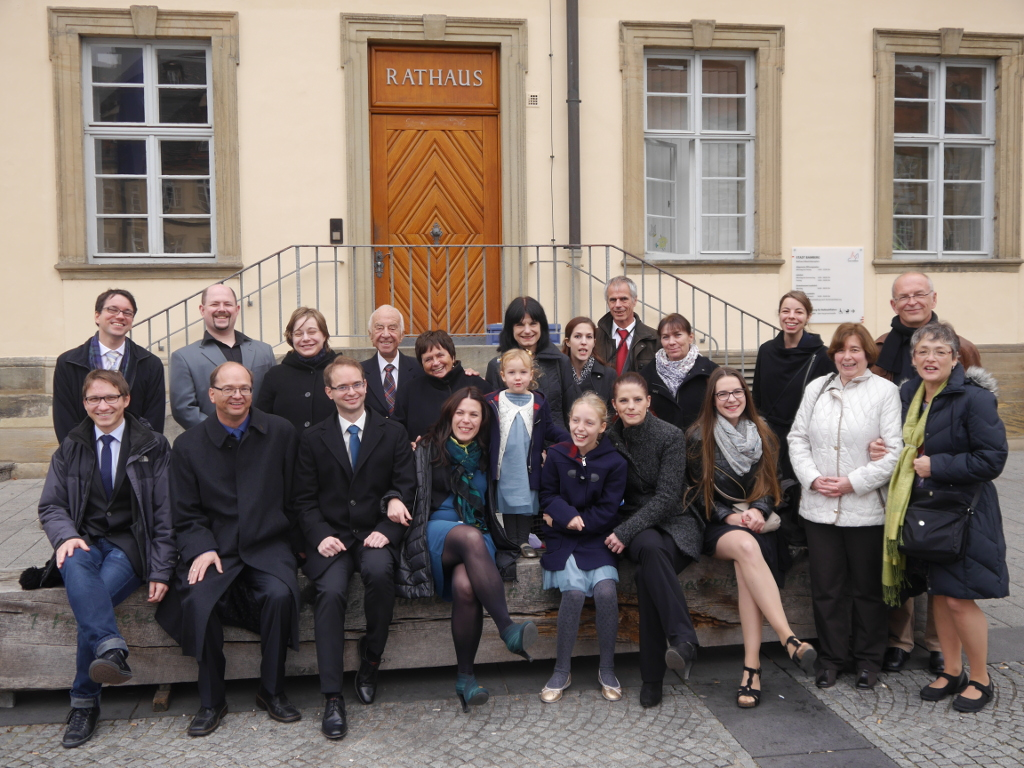
\includegraphics[width=\textwidth]{pic/front.jpg}
	\end{figure}
\LARGE
	\today
\end{titlepage}
\thispagestyle{empty}



\cleardoublepage
\tableofcontents


\cleardoublepage


% background graphic
%\setBackgroundPicture[x, y=-2cm, width=\paperwidth-4cm, height, orientation = pagecenter]{pic/background}

\begin{otherlanguage}{ngerman}
\setHeadlines
{% translation
    inghead = Zutaten,
    prephead = Zubereitung,
    hinthead = Tipp,
    continuationhead = Fortsetzung,
    continuationfoot = Fortsetzung auf n\"achster Seite,
    portionvalue = Personen,
}

%%%%%%%%%%%%%%%%%%%%%%%%%%%%%%%%%%%%%%%%%%%%%%%%%%%%%%%%%%%%%%%%%%%
%				Recipe Section										%
%%%%%%%%%%%%%%%%%%%%%%%%%%%%%%%%%%%%%%%%%%%%%%%%%%%%%%%%%%%%%%%%%%%
\cleardoublepage
\section{Vegetarische Speisen}
\begin{figure}[h]
	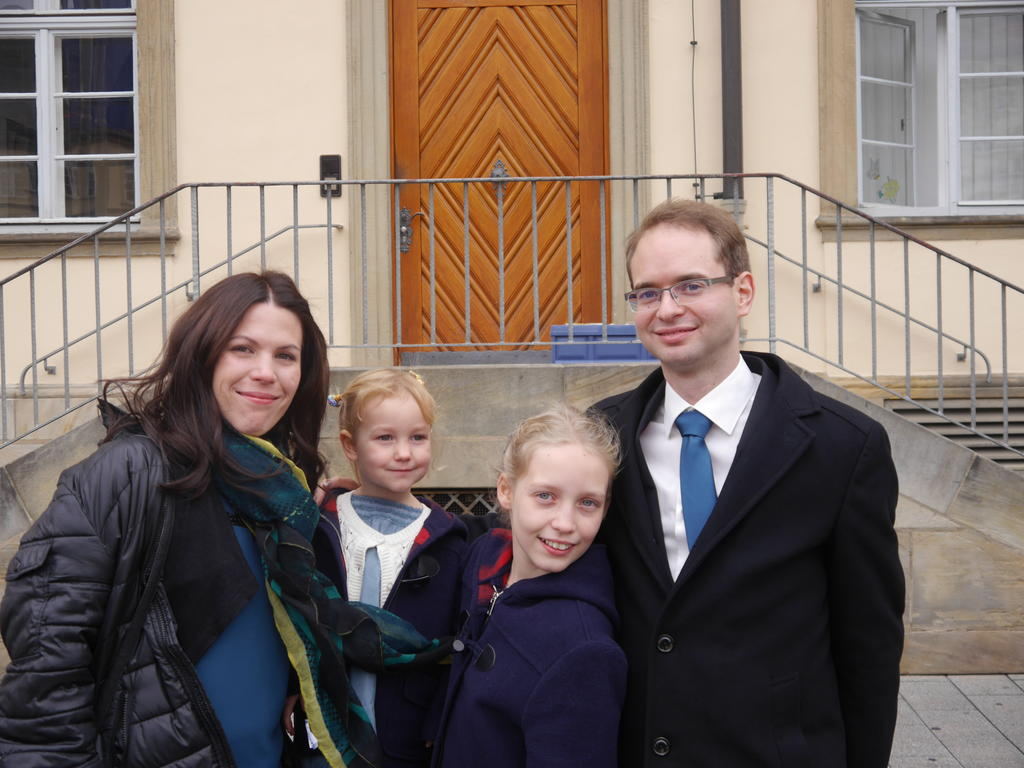
\includegraphics[width=\textwidth]{pic/veggie.jpg}
\end{figure}


\begin{recipe}
[% 
    preparationtime = {\unit[30]{min}},
    portion = {\portion{4}},
    source = {Lieblingsrezept von Ariane (original von chefkoch.de)}
]
{Ratatouille mit Tofu}

    \ingredients{%
        500 g	& 	Tomaten \\
		500 g	& 	Zucchini \\
		500 g &	Paprikaschoten \\
		500 g	&	Aubergine\\
		2	&	Zwiebeln \\
		2	&	Knoblauchzehen \\
		400 g & Räuchertofu \\
		4 EL & Olivenöl\\
		 & Salz und Pfeffer\\
		 2 Stiele & Thymian\\
		2 Stiele & Rosmarin\\
		2 Stiele & Oregano\\
		2 & Lorbeerblatt\\
    }
    
    \preparation{%
    \newline
       \step Das Gemüse gründlich waschen, die Tomaten häuten und in grobe Stücke schneiden. Die Zwiebeln schälen und wie das restliche Gemüse würfeln (ca. erbsengroß). Den Knoblauch schälen und fein hacken. 
       \step Das Olivenöl in einem weiten Topf erhitzen, die Gemüse darin getrennt nach Sorten jeweils 10 Minuten garen, dann herausnehmen (das Gemüse für das Ratatouille getrennt anbraten und erst ganz am Ende miteinander vermischen).
       \step Anschließend den Tofu kurz abtrocknen und würfeln. Das Gemüse vermengen. Die Kräuter mit dem Lorbeerblatt, dem Knoblauch und dem gewürfelten Tofu dazugeben. Mit Salz und Pfeffer würzen und alles weitere 10 Minuten garen.
    }
   
\end{recipe}

\cleardoublepage
\subsection{Herbstrezepte}
\begin{figure}[h]
	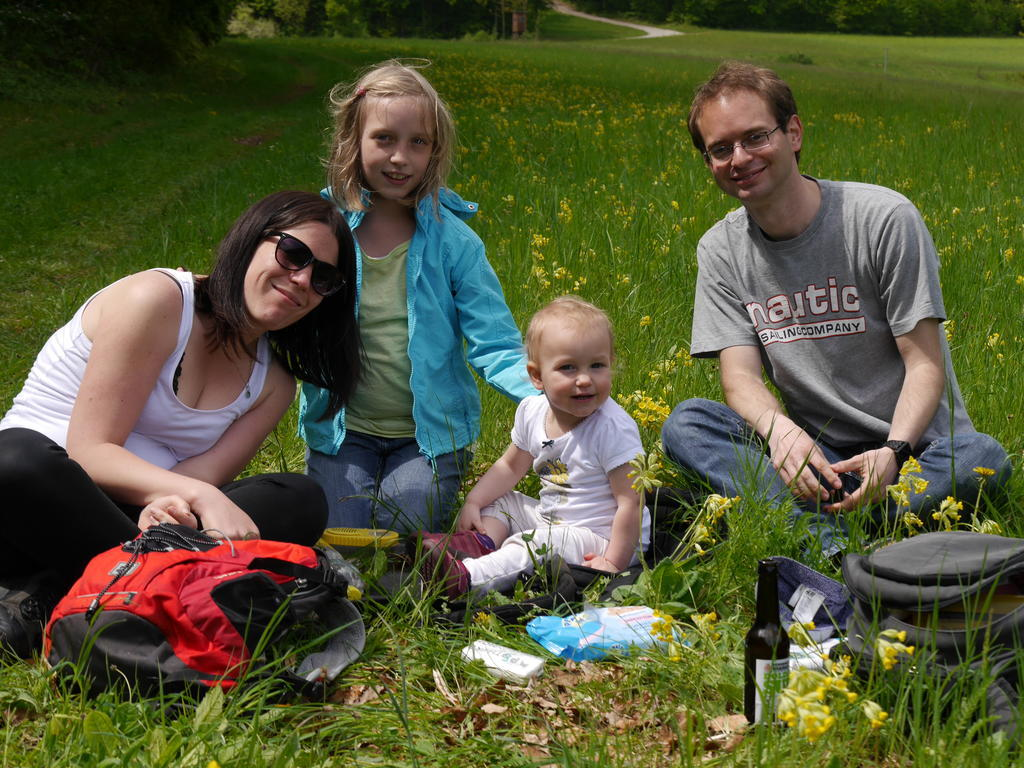
\includegraphics[width=\textwidth]{pic/US}
\end{figure}
\include{recipes/PumpkinSoup}
\include{recipes/CurlyKaleSoup}
\include{recipes/LinsenFenchelEintopf}
\include{recipes/TomatoeBredie}
\include{recipes/BroccoliNoodles}
\include{recipes/MushroomPolenta}
\include{recipes/ColeSlawWok}
\include{recipes/BrokkoliSuesskartoffelAuflauf}
\include{recipes/Cheese}
\include{recipes/AvocadoMouse}


\end{otherlanguage}

\clearpage
~\thispagestyle{empty}
% Last page
\clearpage
\thispagestyle{empty}
~
\vfill
\begin{center}
\begin{tikzpicture}[scale=1.5]
\fill (0,0) -- (-0.2, 0.1) -- (-4, 0) -- (-0.2, -0.1) -- cycle;
\fill (0,0) -- (0.2, 0.1) -- (4, 0) -- (0.2, -0.1) -- cycle;
\fill (0,0) circle (0.1);
\end{tikzpicture}
\end{center}


    Eine hochzeitliche Rezeptesammlung -- Gerichte die wir G"aste lecker finden! Wir hoffen ihr findet die eine oder andere Anregung und denkt beim Kochen und Genießen an uns und das wundersch"one Fest.
    
    Wenn ihr mal ausgeschlafen habt könnt ihr unsere ganzen pull-requests unter \url{https://github.com/whatever4711/cookbook} annehmen.
\end{document} 